\chapter{Análisis de Resultados}
\section{Capturas del programa en ejecución}

A continuación se presenta en orden el proceso de ejecución del programa, donde primeramente se muestra el código en ejecución con un ejemplo de 1 pieza aleatoria, luego de este ejemplo, elegiremos la opción de recorrido para 2 piezas manuales.\newline
\newpage

\begin{enumerate}
\item Iniciamos el programa, donde nos pide que introduzcamos la cantidad de piezas a invocar en el tablero. Para este caso en particular se seleccionó 1 pieza. Ahora nos pide que elegíamos si la pieza generara su recorrido de forma aleatoria o manual, para este caso se seleccionó la opción aleatoria. Luego nos muestra datos sobre la ruta generada aleatoriamente, su respectivo tamaño y el recorrido que se seleccionó de los recorridos\_finales posibles. Finalmente, nos indica que veamos la parte gráfica. Observar la Figura 2.1.

\begin{figure}[h]
\begin{minipage}{0.3\textwidth}
    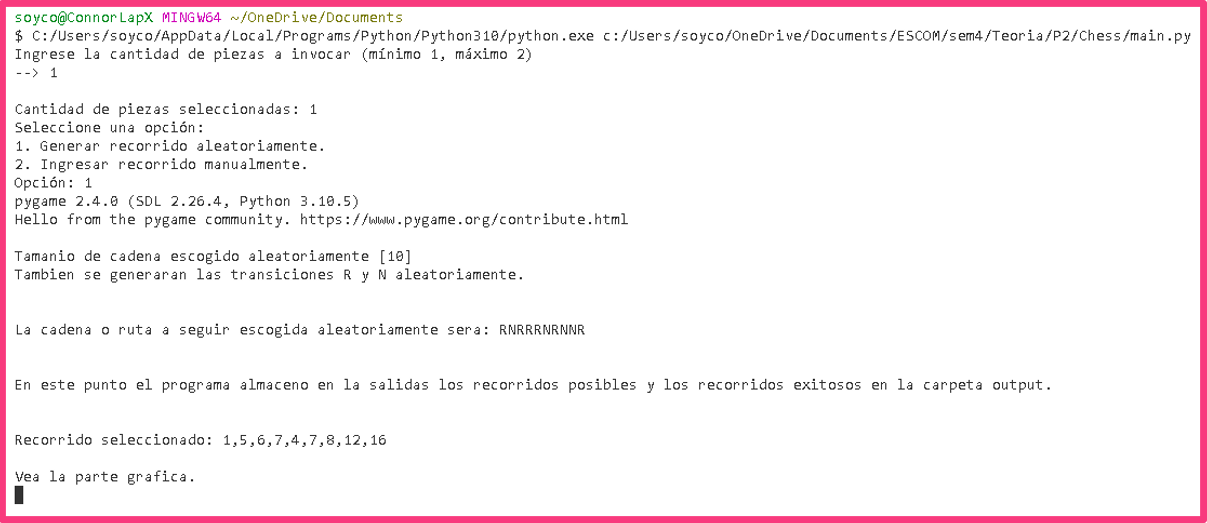
\includegraphics[width=4\linewidth]{Images/Cap1.png}
\end{minipage}
\caption{Inicio del programa en terminal.}
\label{fig:imagen}
\end{figure}
\newpage
\item Aquí podemos ver la salida del archivo recorrido\_blanca.txt y el de recorrido\_finales\_blanca.txt donde en el primero se almacenaron todos los recorridos posibles y en el segundo solo los recorridos que llevan al estado de éxito 16.  Observar la Figura 2.2.\newline
\begin{figure}[h]
%\begin{minipage}{0.3\textwidth}
    \begin{center}
    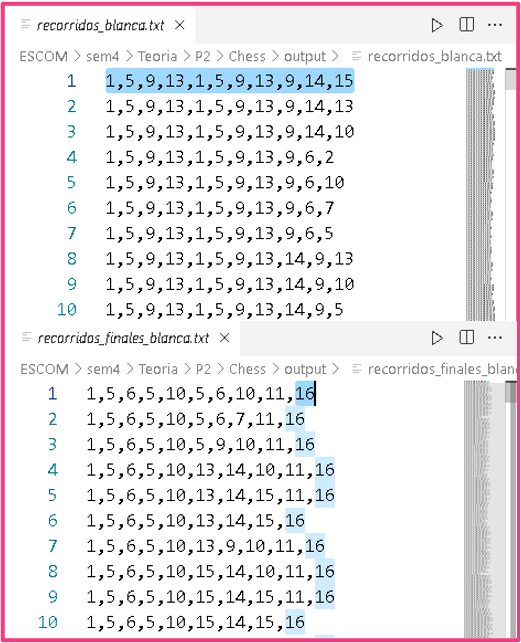
\includegraphics[width=0.7\linewidth]{Images/Cap6.png}
    \end{center}
%\end{minipage}
\caption{Vista de archivos de salida de recorridos.}
\label{fig:imagen}
\end{figure}

\newpage
\item Aquí se puede ver la secuencia que sigue la parte gráfica, donde al dar clic al botón $"$Siguiente$"$ nos lleva al siguiente movimiento. Observar la Figura 2.3.
\begin{figure}[h]
%\begin{minipage}{0.3\textwidth}
    \begin{center}
    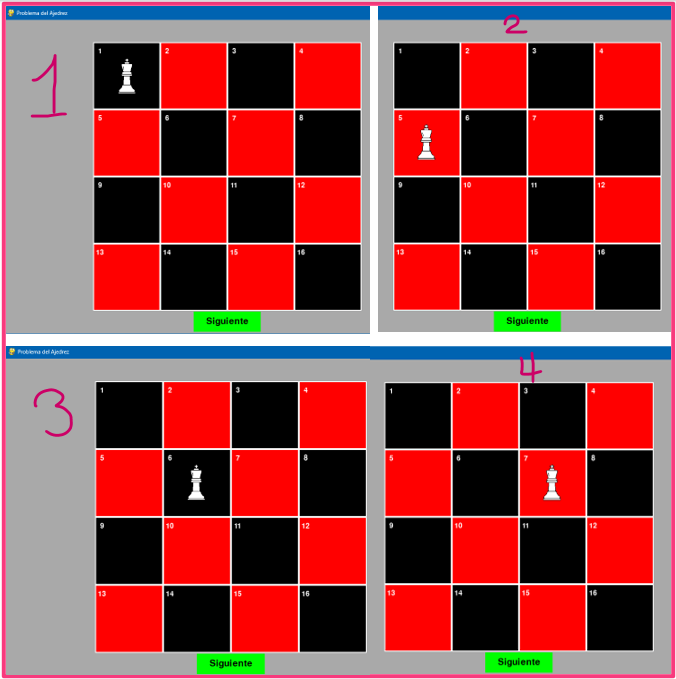
\includegraphics[width=0.8\linewidth]{Images/Cap2.png}
    \end{center}
%\end{minipage}
\caption{Visualización de transiciones gráficas.}
\label{fig:imagen}
\end{figure}

\newpage
\item Siguiente imagen de transiciones graficas. Observar la Figura 2.4.
\begin{figure}[h]
%\begin{minipage}{0.3\textwidth}
    \begin{center}
    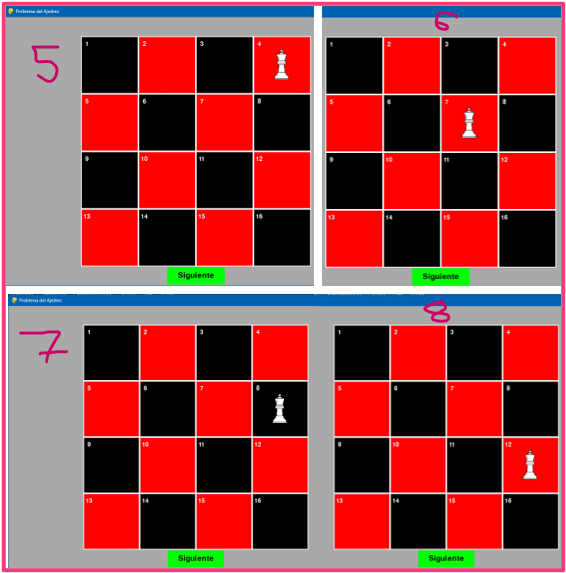
\includegraphics[width=0.7\linewidth]{Images/Cap3.png}
    \end{center}
%\end{minipage}
\caption{Transiciones graficas.}
\label{fig:imagen}
\end{figure}

\newpage
\item Final de la transición gráfica, el programa nos dice que ha terminado. Observar la figura 2.5.

\begin{figure}[h]
%\begin{minipage}{0.3\textwidth}
    \begin{center}
    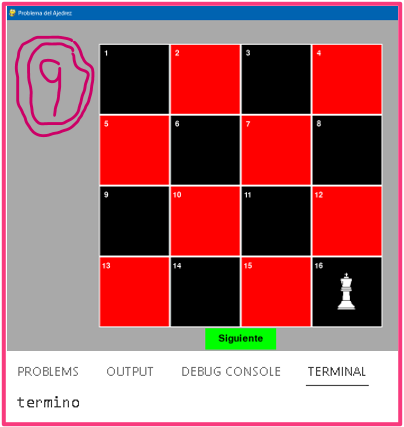
\includegraphics[width=0.7\linewidth]{Images/Cap4.png}
    \end{center}
%\end{minipage}
\caption{Fin de transición y final en terminal.}
\label{fig:imagen}
\end{figure}

\newpage
\item Aquí podemos ver el árbol de recorridos correspondiente al recorrido que se ha escogido aleatoriamente. Observar la figura 2.6.

\begin{figure}[h]
%\begin{minipage}{0.3\textwidth}
    \begin{center}
    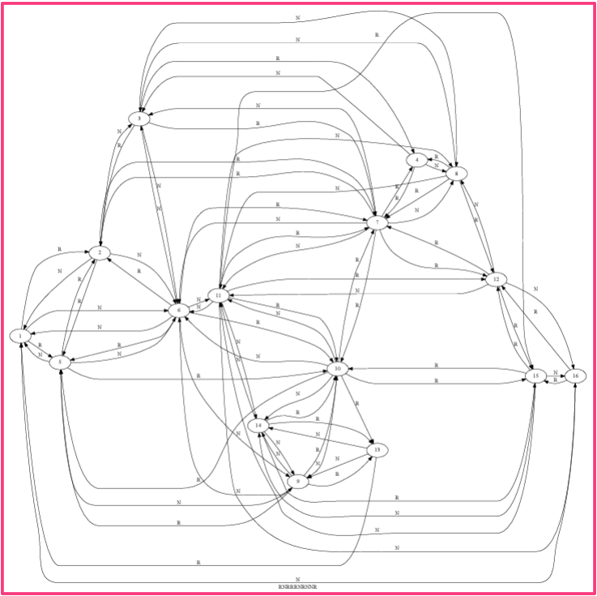
\includegraphics[width=0.7\linewidth]{Images/Cap5.png}
    \end{center}
%\end{minipage}
\caption{Grafo de recorrido.}
\label{fig:imagen}
\end{figure}
\newpage
\item Iniciamos el programa´nuevamente, donde nos pide que introduzcamos la cantidad de piezas a invocar en el tablero. Para este caso en particular se seleccionó 2 piezas. Ahora nos pide que elegíamos entre diferentes configuraciones, elegimos el caso de manual vs manual, que básicamente nosotros introduciremos el recorrido a recorrer. Luego nos muestra datos sobre las rutas seleccionadas aleatoriamente, su respectivo tamaño. Finalmente, nos indica que pieza empieza primero. Podemos observar que la pieza negra colisionará con la pieza blanca cuando esta se recorra al estado 6. Observar la figura 2.7.

\begin{figure}[h]
%\begin{minipage}{0.3\textwidth}
    \begin{center}
    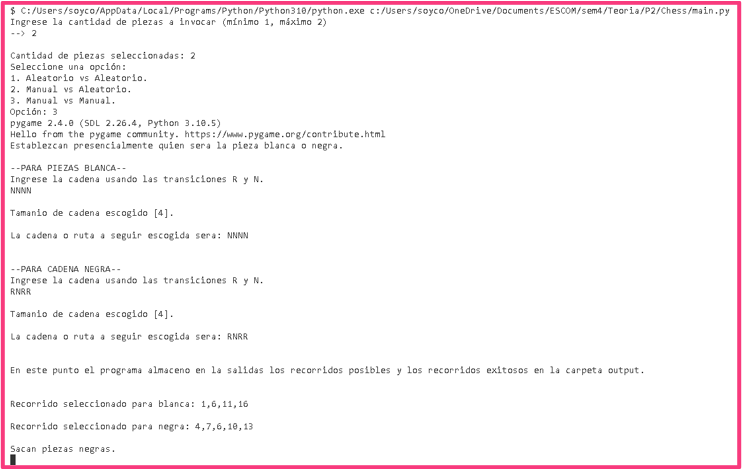
\includegraphics[width=0.8\linewidth]{Images/Cap7.png}
    \end{center}
%\end{minipage}
\caption{Vista de terminal de segundo caso.}
\label{fig:imagen}
\end{figure}
\newpage
\item Pasos de transiciones de la parte gráfica, donde en el último caso de transición se detecta la colisión y se recalcula una ruta. Observar figura 2.8.

\begin{figure}[h]
%\begin{minipage}{0.3\textwidth}
    \begin{center}
    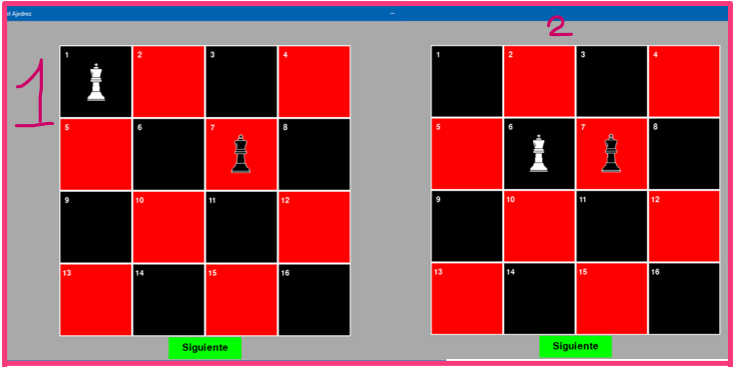
\includegraphics[width=0.8\linewidth]{Images/Cap9.png}
    \end{center}
%\end{minipage}
\caption{Secuencia de transiciones, donde en caso 2 hay colisión.}
\label{fig:imagen}
\end{figure}

\newpage
\item Se detecta una colisión, por ende se reconfigura el recorrido y por ende los recorridos posibles y los recorridos finales, por lo que se vuelve a escoger una ruta adecuada. Observar figura 2.9.

\begin{figure}[h]
%\begin{minipage}{0.3\textwidth}
    \begin{center}
    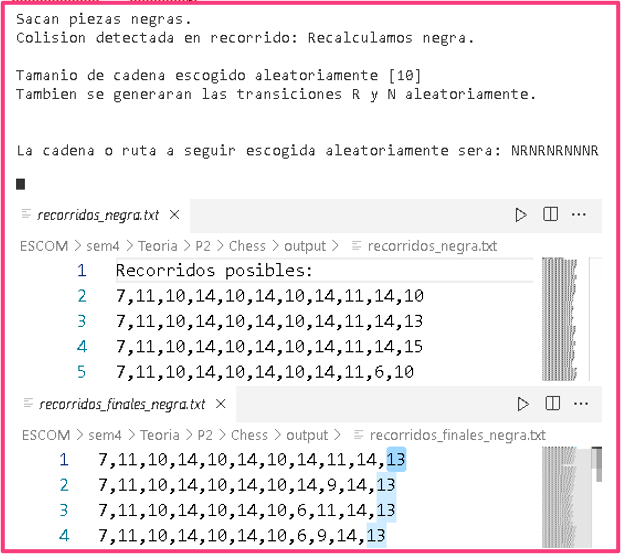
\includegraphics[width=0.8\linewidth]{Images/Cap10.png}
    \end{center}
%\end{minipage}
\caption{Vista de terminal de nueva ruta configurada y salida en archivos.}
\label{fig:imagen}
\end{figure}

\newpage
\item Regresamos a la parte gráfica donde ahora si nos reconfiguró una ruta para la pieza negra, donde podemos ver que la pieza blanca terminó por llegar primero al estado 16 y el juego se acaba. Observar figura 2.10.

\begin{figure}[h]
%\begin{minipage}{0.3\textwidth}
    \begin{center}
    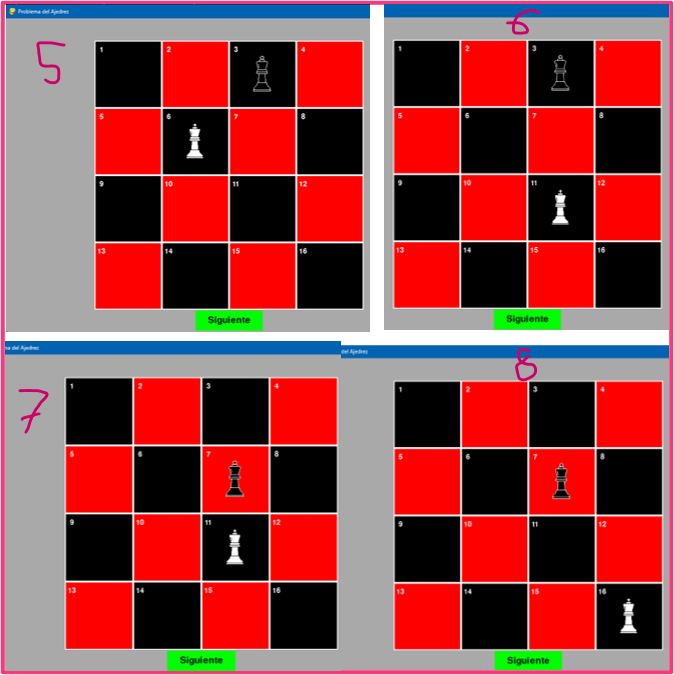
\includegraphics[width=0.8\linewidth]{Images/Cap11.png}
    \end{center}
%\end{minipage}
\caption{Vista de gráfica del ajedrez.}
\label{fig:imagen}
\end{figure}

\newpage
\item Aquí podemos ver la renderización del arbol o grafo de recorridos para pieza blanca.  Observar la figura 2.11.

\begin{figure}[h]
\begin{minipage}{0.3\textwidth}
    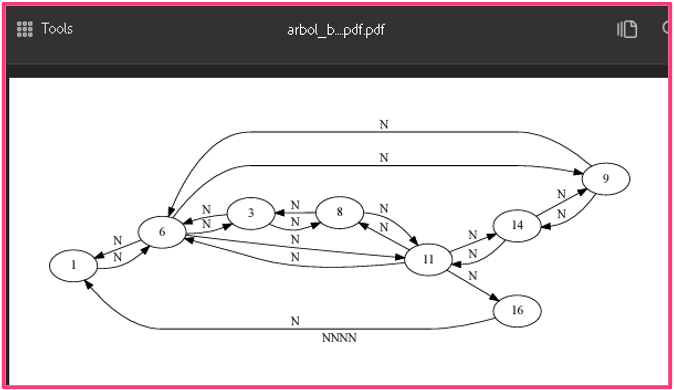
\includegraphics[width=4\linewidth]{Images/Cap12.png}
\end{minipage}
\caption{Árbol de recorridos para pieza blanca.}
\label{fig:imagen}
\end{figure}

\newpage
\item Aquí podemos ver la renderización del arbol o grafo de recorridos para pieza negra. Observar la figura 2.12.

\begin{figure}[h]
\begin{minipage}{0.3\textwidth}
    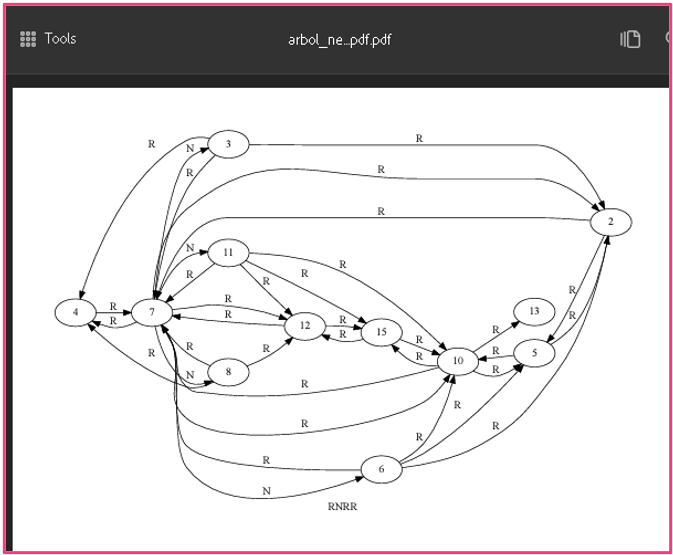
\includegraphics[width=4\linewidth]{Images/Cap13.png}
\end{minipage}
\caption{Árbol de recorridos para pieza negra.}
\label{fig:imagen}
\end{figure}
\newpage
\item Aquí podemos ver el caso para cuando digitamos un recorrido de mayor longitud, para este caso fue una cadena de recorrido de tamaño 82. Observar la figura 2.12.

\begin{figure}[h]
\begin{minipage}{0.3\textwidth}
    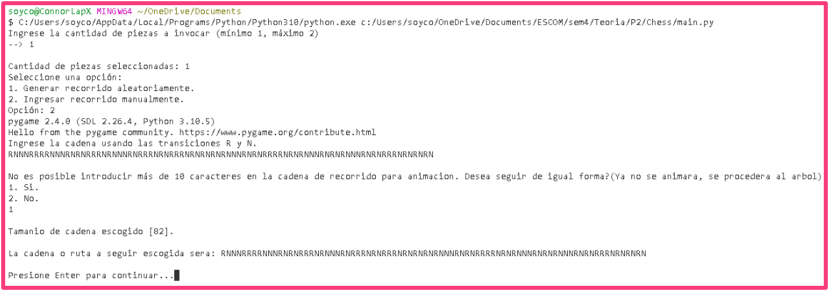
\includegraphics[width=4\linewidth]{Images/Cap14.png}
\end{minipage}
\caption{Vista de terminal para recorrido de tamaño 82.}
\label{fig:imagen}
\end{figure}
\newpage
\item Aquí podemos ver el archivo de recorridos posibles para la pieza, donde el formato de guardado del recorrido se almacena de manera muy distinta, siendo separado cada recorrido por puntos en vez de saltos de línea, para de esta manera evitar una creciente exponencial en la generación del documento. Observar la figura 2.12.

\begin{figure}[h]
\begin{minipage}{0.3\textwidth}
    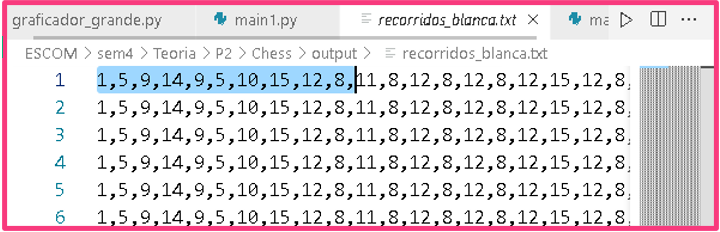
\includegraphics[width=4\linewidth]{Images/Cap15.png}
\end{minipage}
\caption{Vista de archivo de recorridos para la pieza blanca.}
\label{fig:imagen}
\end{figure}
\newpage
\item Grafo de recorridos para la cadena de tamaño 82. Observar la figura 2.12.

\begin{figure}[h]
\begin{minipage}{0.3\textwidth}
    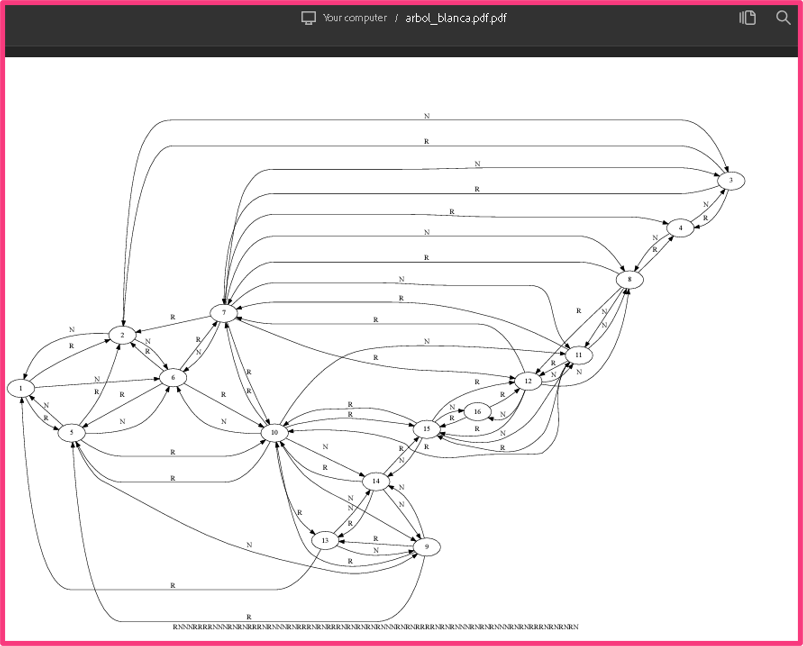
\includegraphics[width=4\linewidth]{Images/Cap16.png}
\end{minipage}
\caption{Árbol de recorridos para pieza en cuestión.}
\label{fig:imagen}
\end{figure}

\end{enumerate}